% Generated by Sphinx.
\def\sphinxdocclass{report}
\documentclass[letterpaper,10pt,english]{sphinxmanual}
\usepackage[utf8]{inputenc}
\DeclareUnicodeCharacter{00A0}{\nobreakspace}
\usepackage{cmap}
\usepackage[T1]{fontenc}
\usepackage{babel}
\usepackage{times}
\usepackage[Bjarne]{fncychap}
\usepackage{longtable}
\usepackage{sphinx}
\usepackage{multirow}


\title{Tango Controls Documentation Documentation}
\date{August 18, 2016}
\release{0.1}
\author{Tango Community, 3Controls, Piotr Goryl}
\newcommand{\sphinxlogo}{}
\renewcommand{\releasename}{Release}
\makeindex

\makeatletter
\def\PYG@reset{\let\PYG@it=\relax \let\PYG@bf=\relax%
    \let\PYG@ul=\relax \let\PYG@tc=\relax%
    \let\PYG@bc=\relax \let\PYG@ff=\relax}
\def\PYG@tok#1{\csname PYG@tok@#1\endcsname}
\def\PYG@toks#1+{\ifx\relax#1\empty\else%
    \PYG@tok{#1}\expandafter\PYG@toks\fi}
\def\PYG@do#1{\PYG@bc{\PYG@tc{\PYG@ul{%
    \PYG@it{\PYG@bf{\PYG@ff{#1}}}}}}}
\def\PYG#1#2{\PYG@reset\PYG@toks#1+\relax+\PYG@do{#2}}

\expandafter\def\csname PYG@tok@gd\endcsname{\def\PYG@tc##1{\textcolor[rgb]{0.63,0.00,0.00}{##1}}}
\expandafter\def\csname PYG@tok@gu\endcsname{\let\PYG@bf=\textbf\def\PYG@tc##1{\textcolor[rgb]{0.50,0.00,0.50}{##1}}}
\expandafter\def\csname PYG@tok@gt\endcsname{\def\PYG@tc##1{\textcolor[rgb]{0.00,0.27,0.87}{##1}}}
\expandafter\def\csname PYG@tok@gs\endcsname{\let\PYG@bf=\textbf}
\expandafter\def\csname PYG@tok@gr\endcsname{\def\PYG@tc##1{\textcolor[rgb]{1.00,0.00,0.00}{##1}}}
\expandafter\def\csname PYG@tok@cm\endcsname{\let\PYG@it=\textit\def\PYG@tc##1{\textcolor[rgb]{0.25,0.50,0.56}{##1}}}
\expandafter\def\csname PYG@tok@vg\endcsname{\def\PYG@tc##1{\textcolor[rgb]{0.73,0.38,0.84}{##1}}}
\expandafter\def\csname PYG@tok@m\endcsname{\def\PYG@tc##1{\textcolor[rgb]{0.13,0.50,0.31}{##1}}}
\expandafter\def\csname PYG@tok@mh\endcsname{\def\PYG@tc##1{\textcolor[rgb]{0.13,0.50,0.31}{##1}}}
\expandafter\def\csname PYG@tok@cs\endcsname{\def\PYG@tc##1{\textcolor[rgb]{0.25,0.50,0.56}{##1}}\def\PYG@bc##1{\setlength{\fboxsep}{0pt}\colorbox[rgb]{1.00,0.94,0.94}{\strut ##1}}}
\expandafter\def\csname PYG@tok@ge\endcsname{\let\PYG@it=\textit}
\expandafter\def\csname PYG@tok@vc\endcsname{\def\PYG@tc##1{\textcolor[rgb]{0.73,0.38,0.84}{##1}}}
\expandafter\def\csname PYG@tok@il\endcsname{\def\PYG@tc##1{\textcolor[rgb]{0.13,0.50,0.31}{##1}}}
\expandafter\def\csname PYG@tok@go\endcsname{\def\PYG@tc##1{\textcolor[rgb]{0.20,0.20,0.20}{##1}}}
\expandafter\def\csname PYG@tok@cp\endcsname{\def\PYG@tc##1{\textcolor[rgb]{0.00,0.44,0.13}{##1}}}
\expandafter\def\csname PYG@tok@gi\endcsname{\def\PYG@tc##1{\textcolor[rgb]{0.00,0.63,0.00}{##1}}}
\expandafter\def\csname PYG@tok@gh\endcsname{\let\PYG@bf=\textbf\def\PYG@tc##1{\textcolor[rgb]{0.00,0.00,0.50}{##1}}}
\expandafter\def\csname PYG@tok@ni\endcsname{\let\PYG@bf=\textbf\def\PYG@tc##1{\textcolor[rgb]{0.84,0.33,0.22}{##1}}}
\expandafter\def\csname PYG@tok@nl\endcsname{\let\PYG@bf=\textbf\def\PYG@tc##1{\textcolor[rgb]{0.00,0.13,0.44}{##1}}}
\expandafter\def\csname PYG@tok@nn\endcsname{\let\PYG@bf=\textbf\def\PYG@tc##1{\textcolor[rgb]{0.05,0.52,0.71}{##1}}}
\expandafter\def\csname PYG@tok@no\endcsname{\def\PYG@tc##1{\textcolor[rgb]{0.38,0.68,0.84}{##1}}}
\expandafter\def\csname PYG@tok@na\endcsname{\def\PYG@tc##1{\textcolor[rgb]{0.25,0.44,0.63}{##1}}}
\expandafter\def\csname PYG@tok@nb\endcsname{\def\PYG@tc##1{\textcolor[rgb]{0.00,0.44,0.13}{##1}}}
\expandafter\def\csname PYG@tok@nc\endcsname{\let\PYG@bf=\textbf\def\PYG@tc##1{\textcolor[rgb]{0.05,0.52,0.71}{##1}}}
\expandafter\def\csname PYG@tok@nd\endcsname{\let\PYG@bf=\textbf\def\PYG@tc##1{\textcolor[rgb]{0.33,0.33,0.33}{##1}}}
\expandafter\def\csname PYG@tok@ne\endcsname{\def\PYG@tc##1{\textcolor[rgb]{0.00,0.44,0.13}{##1}}}
\expandafter\def\csname PYG@tok@nf\endcsname{\def\PYG@tc##1{\textcolor[rgb]{0.02,0.16,0.49}{##1}}}
\expandafter\def\csname PYG@tok@si\endcsname{\let\PYG@it=\textit\def\PYG@tc##1{\textcolor[rgb]{0.44,0.63,0.82}{##1}}}
\expandafter\def\csname PYG@tok@s2\endcsname{\def\PYG@tc##1{\textcolor[rgb]{0.25,0.44,0.63}{##1}}}
\expandafter\def\csname PYG@tok@vi\endcsname{\def\PYG@tc##1{\textcolor[rgb]{0.73,0.38,0.84}{##1}}}
\expandafter\def\csname PYG@tok@nt\endcsname{\let\PYG@bf=\textbf\def\PYG@tc##1{\textcolor[rgb]{0.02,0.16,0.45}{##1}}}
\expandafter\def\csname PYG@tok@nv\endcsname{\def\PYG@tc##1{\textcolor[rgb]{0.73,0.38,0.84}{##1}}}
\expandafter\def\csname PYG@tok@s1\endcsname{\def\PYG@tc##1{\textcolor[rgb]{0.25,0.44,0.63}{##1}}}
\expandafter\def\csname PYG@tok@gp\endcsname{\let\PYG@bf=\textbf\def\PYG@tc##1{\textcolor[rgb]{0.78,0.36,0.04}{##1}}}
\expandafter\def\csname PYG@tok@sh\endcsname{\def\PYG@tc##1{\textcolor[rgb]{0.25,0.44,0.63}{##1}}}
\expandafter\def\csname PYG@tok@ow\endcsname{\let\PYG@bf=\textbf\def\PYG@tc##1{\textcolor[rgb]{0.00,0.44,0.13}{##1}}}
\expandafter\def\csname PYG@tok@sx\endcsname{\def\PYG@tc##1{\textcolor[rgb]{0.78,0.36,0.04}{##1}}}
\expandafter\def\csname PYG@tok@bp\endcsname{\def\PYG@tc##1{\textcolor[rgb]{0.00,0.44,0.13}{##1}}}
\expandafter\def\csname PYG@tok@c1\endcsname{\let\PYG@it=\textit\def\PYG@tc##1{\textcolor[rgb]{0.25,0.50,0.56}{##1}}}
\expandafter\def\csname PYG@tok@kc\endcsname{\let\PYG@bf=\textbf\def\PYG@tc##1{\textcolor[rgb]{0.00,0.44,0.13}{##1}}}
\expandafter\def\csname PYG@tok@c\endcsname{\let\PYG@it=\textit\def\PYG@tc##1{\textcolor[rgb]{0.25,0.50,0.56}{##1}}}
\expandafter\def\csname PYG@tok@mf\endcsname{\def\PYG@tc##1{\textcolor[rgb]{0.13,0.50,0.31}{##1}}}
\expandafter\def\csname PYG@tok@err\endcsname{\def\PYG@bc##1{\setlength{\fboxsep}{0pt}\fcolorbox[rgb]{1.00,0.00,0.00}{1,1,1}{\strut ##1}}}
\expandafter\def\csname PYG@tok@mb\endcsname{\def\PYG@tc##1{\textcolor[rgb]{0.13,0.50,0.31}{##1}}}
\expandafter\def\csname PYG@tok@ss\endcsname{\def\PYG@tc##1{\textcolor[rgb]{0.32,0.47,0.09}{##1}}}
\expandafter\def\csname PYG@tok@sr\endcsname{\def\PYG@tc##1{\textcolor[rgb]{0.14,0.33,0.53}{##1}}}
\expandafter\def\csname PYG@tok@mo\endcsname{\def\PYG@tc##1{\textcolor[rgb]{0.13,0.50,0.31}{##1}}}
\expandafter\def\csname PYG@tok@kd\endcsname{\let\PYG@bf=\textbf\def\PYG@tc##1{\textcolor[rgb]{0.00,0.44,0.13}{##1}}}
\expandafter\def\csname PYG@tok@mi\endcsname{\def\PYG@tc##1{\textcolor[rgb]{0.13,0.50,0.31}{##1}}}
\expandafter\def\csname PYG@tok@kn\endcsname{\let\PYG@bf=\textbf\def\PYG@tc##1{\textcolor[rgb]{0.00,0.44,0.13}{##1}}}
\expandafter\def\csname PYG@tok@o\endcsname{\def\PYG@tc##1{\textcolor[rgb]{0.40,0.40,0.40}{##1}}}
\expandafter\def\csname PYG@tok@kr\endcsname{\let\PYG@bf=\textbf\def\PYG@tc##1{\textcolor[rgb]{0.00,0.44,0.13}{##1}}}
\expandafter\def\csname PYG@tok@s\endcsname{\def\PYG@tc##1{\textcolor[rgb]{0.25,0.44,0.63}{##1}}}
\expandafter\def\csname PYG@tok@kp\endcsname{\def\PYG@tc##1{\textcolor[rgb]{0.00,0.44,0.13}{##1}}}
\expandafter\def\csname PYG@tok@w\endcsname{\def\PYG@tc##1{\textcolor[rgb]{0.73,0.73,0.73}{##1}}}
\expandafter\def\csname PYG@tok@kt\endcsname{\def\PYG@tc##1{\textcolor[rgb]{0.56,0.13,0.00}{##1}}}
\expandafter\def\csname PYG@tok@sc\endcsname{\def\PYG@tc##1{\textcolor[rgb]{0.25,0.44,0.63}{##1}}}
\expandafter\def\csname PYG@tok@sb\endcsname{\def\PYG@tc##1{\textcolor[rgb]{0.25,0.44,0.63}{##1}}}
\expandafter\def\csname PYG@tok@k\endcsname{\let\PYG@bf=\textbf\def\PYG@tc##1{\textcolor[rgb]{0.00,0.44,0.13}{##1}}}
\expandafter\def\csname PYG@tok@se\endcsname{\let\PYG@bf=\textbf\def\PYG@tc##1{\textcolor[rgb]{0.25,0.44,0.63}{##1}}}
\expandafter\def\csname PYG@tok@sd\endcsname{\let\PYG@it=\textit\def\PYG@tc##1{\textcolor[rgb]{0.25,0.44,0.63}{##1}}}

\def\PYGZbs{\char`\\}
\def\PYGZus{\char`\_}
\def\PYGZob{\char`\{}
\def\PYGZcb{\char`\}}
\def\PYGZca{\char`\^}
\def\PYGZam{\char`\&}
\def\PYGZlt{\char`\<}
\def\PYGZgt{\char`\>}
\def\PYGZsh{\char`\#}
\def\PYGZpc{\char`\%}
\def\PYGZdl{\char`\$}
\def\PYGZhy{\char`\-}
\def\PYGZsq{\char`\'}
\def\PYGZdq{\char`\"}
\def\PYGZti{\char`\~}
% for compatibility with earlier versions
\def\PYGZat{@}
\def\PYGZlb{[}
\def\PYGZrb{]}
\makeatother

\renewcommand\PYGZsq{\textquotesingle}

\begin{document}

\maketitle
\tableofcontents
\phantomsection\label{index::doc}
{\hfill
\includegraphics{logo_tangocontrols.png}\hfill}



Contents:


\chapter{Tango on Windows}
\label{tango-on-windows:tango-on-windows}\label{tango-on-windows::doc}\label{tango-on-windows:welcome-to-tango-controls-documentation}
This guide provides step by step guide on installation of Tango Controls under Windows operating systems.


\section{What is Tango Controls}
\label{tango-on-windows:what-is-tango-controls}
Tango Controls is an object oriented, distributed control system. It is a framework for building custom SCADA systems.
It defines communication protocol and API. It provides libraries, set of GUI tools and drivers (so called
{\hyperref[glossary:term-device-servers]{\emph{Device Servers}}}) for variety of standard and specific control equipment. For more information see:
\href{http://www.tango-controls.org/what-is-tango-controls/}{http://www.tango-controls.org/what-is-tango-controls/}

{\hfill
\includegraphics{logo_tangocontrols.png}\hfill}

Your computer may have different (one or more) roles in the Tango CS system. The roles are:
\begin{itemize}
\item {} 
Client computer, where you run GUI applications like \textbf{Synoptic},

\item {} 
Tango Host, where configuration of all other components is stored,

\item {} 
Device Servers running.

\end{itemize}

Your Windows computer may perform all above roles simultaneously.


\section{Tango  package installation}
\label{tango-on-windows:tango-package-installation}\setbox0\vbox{
\begin{minipage}{0.95\linewidth}
\textbf{Prerequisite}

\medskip


Some \textbf{Tango Controls} tools require \textbf{Java Runtime Environment (JRE) \textgreater{}=1.7}. Please install it first.
You may find JRE on \href{http://java.com}{http://java.com} .
\end{minipage}}
\begin{center}\setlength{\fboxsep}{5pt}\shadowbox{\box0}\end{center}

The simplest way to have Tango Controls running is to install it from a binary package. Binaries are available at
\href{http://www.tango-controls.org/downloads/binary/}{http://www.tango-controls.org/downloads/binary/}
\begin{itemize}
\item {} 
Download the binary package with your favorite browser.

\end{itemize}
\setbox0\vbox{
\begin{minipage}{0.95\linewidth}
\textbf{Tango Host, DataBaseds}

\medskip


Each Tango Controls system/deployment has to have at least one running DataBaseds {\hyperref[glossary:term-device-server]{\emph{Device Server}}}. The machine
on which the {\hyperref[glossary:term-device-server]{\emph{Device Server}}} is running has a role of so called {\hyperref[glossary:term-tango-host]{\emph{Tango Host}}}. DataBaseds is a device server providing
configuration information to all other components of the system as well as a runtime catalog of the components/devices. It
allows (among others) client applications to find devices in distributed environment.

The \index{TANGO\_HOST}\index{environment variable!TANGO\_HOST}\code{TANGO\_HOST} variable is providing information about the address or IP number and the port on which the DataBaseds is
listening for connections. The \index{TANGO\_HOST}\index{environment variable!TANGO\_HOST}\code{TANGO\_HOST} environment variable is built as follows:

\emph{host\_name\_or\_IP:port}, example: \code{localhost:10000}
\end{minipage}}
\begin{center}\setlength{\fboxsep}{5pt}\shadowbox{\box0}\end{center}
\begin{itemize}
\item {} 
Run the downloaded executable file (double-click on it when downloaded).

\item {} 
Follow instructions provided by the installation wizard.

\item {} \begin{description}
\item[{Configure \index{TANGO\_HOST}\index{environment variable!TANGO\_HOST}\code{TANGO\_HOST} environment variable:}] \leavevmode\begin{itemize}
\item {} \begin{description}
\item[{On Windows 8 and 10:}] \leavevmode\begin{itemize}
\item {} 
From the Desktop, right-click the very bottom left corner of the screen to get
the \emph{Power User Task Menu}.

\item {} 
From the \emph{Power User Task Menu}, click \emph{System}.

\end{itemize}

\end{description}

\item {} \begin{description}
\item[{On Windows XP and 7}] \leavevmode\begin{itemize}
\item {} 
From the Desktop, right-click the \emph{Computer} icon and select \emph{Properties}. If you
don't have a \emph{Computer} icon on your desktop, click \emph{Start} button, right-click the
\emph{Computer} option in the \emph{Start} menu, and select \emph{Properties}.

\end{itemize}

\end{description}

\item {} 
Click the \emph{Advanced System Settings} link in the left column.

\item {} 
In the System Properties window, click on the \emph{Advanced} tab,
then click the \emph{Environment Variables} button near the bottom of that tab.

\item {} 
In the \emph{Environment Variables} window click the \emph{New} button.

\item {} 
In the field \emph{Name} write \code{TANGO\_HOST}.

\item {} 
In the field \emph{Value} write proper value. If it is the only computer in the Tango System provide \code{localhost:10000}.

\end{itemize}

\end{description}

\end{itemize}

If there is a {\hyperref[glossary:term-tango-host]{\emph{Tango Host}}} already running on some other computer in your deployment and you have provided proper
address and port in the \index{TANGO\_HOST}\index{environment variable!TANGO\_HOST}\code{TANGO\_HOST} you may start using client and management applications like
\textbf{Jive}, \textbf{Jdraw}/\textbf{Synoptic}. In other case you have to configure the system to perform a role of
{\hyperref[glossary:term-tango-host]{\emph{Tango Host}}}.


\section{Tango Host role}
\label{tango-on-windows:tango-host-role}
Tango Host role is created by running the \textbf{DataBaseds} device server. This device server requires MySQL
database in its most common application. To make a computer become a Tango Host you need to:
\begin{itemize}
\item {} \begin{description}
\item[{Install MySQL server.}] \leavevmode
You may use community version available from \href{http://dev.mysql.com/downloads/mysql/}{http://dev.mysql.com/downloads/mysql/} . It is suggested to use
\textbf{MySQL Installer} with all tools included. You may read more on MySQL installation topic here:
\href{http://dev.mysql.com/doc/refman/5.7/en/windows-installation.html}{http://dev.mysql.com/doc/refman/5.7/en/windows-installation.html}

It is suggested to create dedicated \code{tango} user with \emph{DB Admin} priviledges during installation.
In the installation wizard on a tab \emph{Accounts and Roles} select button \emph{Add User}
and create a dedicated user. See
\begin{quote}

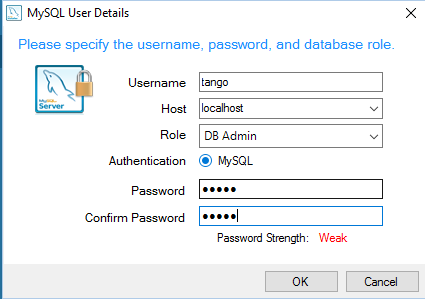
\includegraphics{mysql-user-02.png}
\end{quote}

\end{description}

\item {} \begin{description}
\item[{Setup environment variables providing credentials to access MySQL:}] \leavevmode\begin{itemize}
\item {} 
Open \emph{Command Line}.

\item {} 
Invoke command: \textbf{\%TANGO\_ROOT\%bindbconfig.exe}.
\begin{quote}

\begin{notice}{note}{Note:}
This lets you setup two environment variables
\index{MYSQL\_USER}\index{environment variable!MYSQL\_USER}\code{MYSQL\_USER} and \index{MYSQL\_PASSWORD}\index{environment variable!MYSQL\_PASSWORD}\code{MYSQL\_PASSWORD} used to access the MySQL server. You may use \code{root} credentials
provided upon MySQL installation if it is your development workstation. For production environment it is
suggested to create an additional user with \code{DB Admin} privileges. On Windows you may use \textbf{MySQL Installer}
from \emph{Start} menu and select the option \emph{Reconfigure} for MySQL Server.
Please refer to: \href{http://dev.mysql.com/doc/refman/5.7/en/adding-users.html}{http://dev.mysql.com/doc/refman/5.7/en/adding-users.html}
\end{notice}
\end{quote}

\end{itemize}

\end{description}

\item {} \begin{description}
\item[{Populate database with an initial Tango configuration:}] \leavevmode\begin{itemize}
\item {} 
Open a command line.

\item {} 
Add MySQL client to be available in the PATH. For MySQL version 5.7 the command should be:
\textbf{set PATH=\%PATH\%;''C:Program FilesMySQLMySQL Server 5.7bin''}

\begin{notice}{note}{Note:}
Adjust the path according to your MySQL version and the path where it is installed.
\end{notice}

\item {} 
Invoke \textbf{cd ``\%TANGO\_ROOT\%sharetangodb''}.

\item {} 
Call \textbf{create\_db.bat}.

\end{itemize}

\end{description}

\item {} \begin{description}
\item[{Start a \textbf{DataBaseds} {\hyperref[glossary:term-device-server]{\emph{Device Server}}}:}] \leavevmode\begin{itemize}
\item {} 
Open a new command line window.

\item {} 
In the command line call \textbf{``\%TANGO\_ROOT\%binstart-db.bat''}.
\begin{quote}

\begin{notice}{note}{Note:}
To make your Tango installation operational you have to have this \textbf{DataBaseds} running permanently.
You may either add the command above to \emph{Autostart} or run it as a service.
\end{notice}
\end{quote}

\end{itemize}

\end{description}

\item {} \begin{description}
\item[{Make \textbf{DataBaseds} run as a service}] \leavevmode
\begin{notice}{note}{Note:}
The proposed solution uses NSSM tool which works on all versions of Windows but you may find some other tools
available including native srvany.exe.
\end{notice}
\begin{itemize}
\item {} 
Download NSSM from \href{http://nssm.cc/}{http://nssm.cc/}.

\item {} 
Unpack the file to some convinient location. It is suggested to copy proper (32bit or 64bit) version to the
Tango bin folder \code{\%TANGO\_ROOT\%\textbackslash{}bin\textbackslash{}}.

\item {} 
Open \emph{Command Line} as Administrator.

\item {} 
Change current path to where the \textbf{nssm} is unpacked or copied, eg. \textbf{cd ``\%TANGO\_ROOT\%bin''}.

\item {} \begin{description}
\item[{Invoke \textbf{nssm.exe install Tango-DataBaseds}. This will open a window where you can define service parameters.}] \leavevmode\begin{itemize}
\item {} \begin{description}
\item[{In the Application tab provide information as follows (adjust if your installation path is different).}] \leavevmode
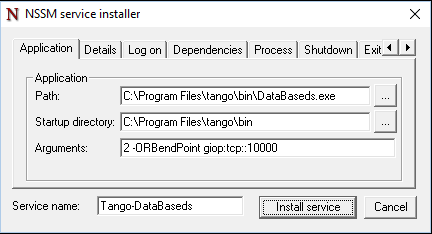
\includegraphics{databaseds-as-service-01.png}

\end{description}

\item {} \begin{description}
\item[{In the Environment tab provide variables with credentials used for accessing the MySQL, like:}] \leavevmode
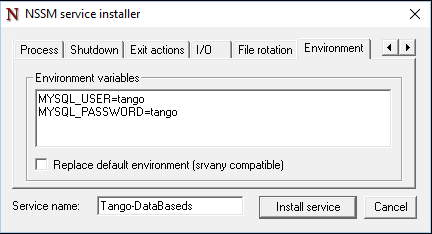
\includegraphics{databaseds-as-service-02.png}

\end{description}

\item {} 
Click \emph{Install Service}.

\end{itemize}

\end{description}

\item {} 
Invoke \textbf{nssm.exe start Tango-DataBaseds} to start the service.

\item {} 
Test if everything is ok. Use \emph{Start} menu to run Jive or in command line call
\textbf{``\%TANGO\_ROOT\%binstart-jive.bat''}.

\end{itemize}

\end{description}

\end{itemize}


\section{Running \emph{Device Servers}}
\label{tango-on-windows:running-device-servers}
The recommended way of running device servers is to use \textbf{Starter} service. Then you may use
\textbf{NSSM} as for \textbf{DataBaseds}.
Assuming you have downloaded it and copied to the Tango bin folder please follow:
\begin{itemize}
\item {} 
Open Command Line as Administrator (if it is not yet open).

\item {} 
Prepare folder for {\hyperref[glossary:term-device-servers]{\emph{Device Servers}}} executable:
\begin{quote}

\begin{notice}{note}{Note:}
To let your device servers start with \textbf{Starter} service their executables have to be in a path without
spaces. This is a limitation of the current \textbf{Starter} implementation.
\end{notice}
\begin{itemize}
\item {} 
Create a directory for {\hyperref[glossary:term-device-servers]{\emph{Device Servers}}}. Let it be \code{C:\textbackslash{}DeviceServers\textbackslash{}bin}
with \textbf{mkdir c:DeviceServersbin}

\item {} 
Change to the Tango bin directory with command (\textbf{cd ``\%TANGO\_ROOT\%bin''})

\item {} 
Copy \textbf{TangoTest} {\hyperref[glossary:term-device-server]{\emph{Device Server}}} to the newly crated folder:
\textbf{copy TangoTest.exe c:DeviceServersbin}

\end{itemize}
\end{quote}

\item {} \begin{description}
\item[{Add entry about the Starter device server you will start on your computer:}] \leavevmode\begin{itemize}
\item {} 
Start a tool called \textbf{Astor}. You may use either Windows \emph{Start} menu or
call \textbf{tango-astor.bat}

\item {} 
In \emph{Astor} window select menu \emph{\DUspan{accelerator}{C}ommand \(\rightarrow\) Add a New Host}

\item {} \begin{description}
\item[{In the form that appears provide your \emph{Host name} and \emph{Device Servers PATH}.}] \leavevmode
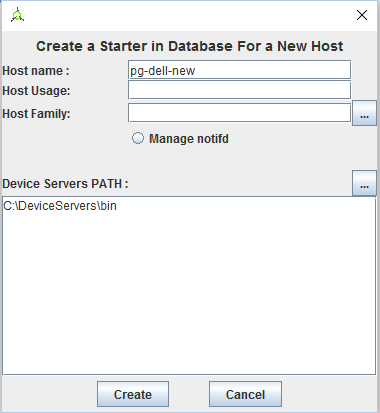
\includegraphics{starter-01.png}

\end{description}

\item {} 
Accept with \emph{Create}

\item {} 
Go back to \textbf{Command Line}

\end{itemize}

\end{description}

\item {} \begin{description}
\item[{Install Starter service:}] \leavevmode\begin{itemize}
\item {} 
Invoke \textbf{nssm.exe install Tango-DataBaseds}.

\item {} 
In the Application tab provide information as follows:
\begin{quote}

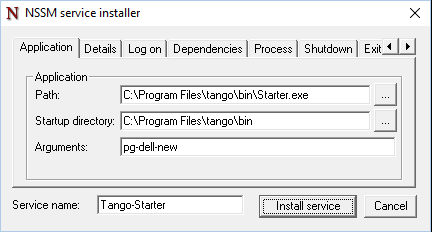
\includegraphics{starter-as-service-01.png}
\end{quote}

\end{itemize}

Adjust if your installation path is different. In \emph{Arguments} exchange \code{pg-dell-new} with the proper name
of your host.
\begin{itemize}
\item {} 
In the Environment tab provide TANGO\_HOST variable, like:
\begin{quote}

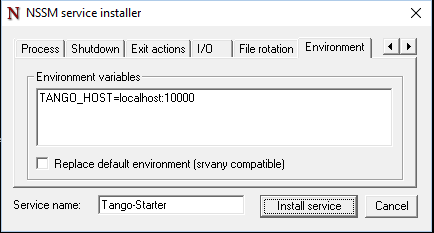
\includegraphics{starter-as-service-02.png}
\end{quote}

\item {} 
Click :guilabel:.

\item {} 
Start the service: \textbf{nssm.exe start Tango-Starter}.

\item {} 
Go back to \textbf{Astor}.

\item {} 
After a while you will see a green led next to your host name:
\begin{quote}

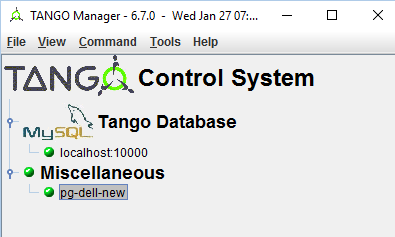
\includegraphics{starter-02.png}
\end{quote}

\end{itemize}

\end{description}

\item {} 
Run \textbf{TangoTest} device server:
\begin{quote}

You may test the configuration by starting prefigured TangoTest device.
\begin{itemize}
\item {} 
Start \textbf{Astor} if it is not running.
\begin{quote}

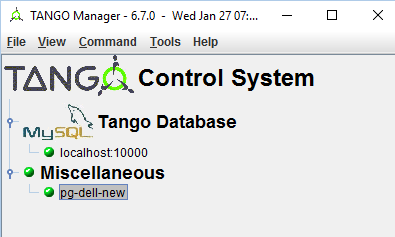
\includegraphics{device-server-01.png}
\end{quote}

\item {} 
Double Click on your computer name to open \emph{Control Panel}. It opens a window as below:
\begin{quote}

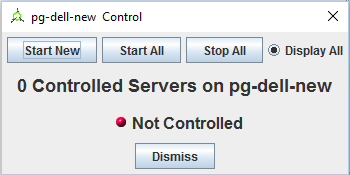
\includegraphics{device-server-02.png}
\end{quote}

\item {} 
Click \emph{Start new}.

\item {} 
In the open window select \emph{TangoTest/test}:
\begin{quote}

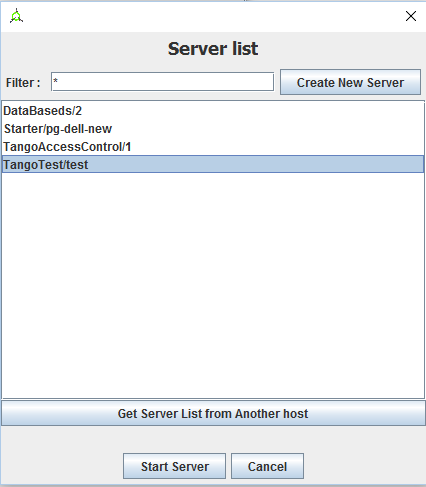
\includegraphics{device-server-03.png}
\end{quote}

\item {} 
Click \emph{Start Server}.

\item {} 
In the open window select \emph{Controlled by Astro -\textgreater{} Yes}, and \emph{Startup Level -\textgreater{} Level 1}.
\begin{quote}

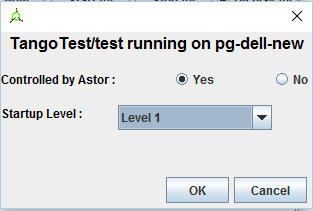
\includegraphics{device-server-04.png}
\end{quote}

\item {} 
When you click \emph{OK} it should start the server. After a while you should see:
\begin{quote}

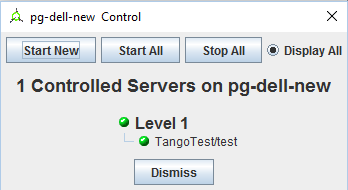
\includegraphics{device-server-05.png}
\end{quote}

\end{itemize}
\end{quote}

\item {} \begin{description}
\item[{Running your {\hyperref[glossary:term-device-servers]{\emph{Device Servers}}}:}] \leavevmode\begin{itemize}
\item {} 
You need to copy an executable to the folder configured for \textbf{Starter}. In our example it is
\code{C:DeviceServersbin}.

\item {} 
Then use \textbf{Astor}. After opening \emph{Control panel} for your computer (double clicking on a label)
and selection \emph{Start New}...

\item {} 
Select \emph{Create New Server} and follow a wizard.

\end{itemize}

\end{description}

\end{itemize}


\section{What's next}
\label{tango-on-windows:what-s-next}\begin{quote}

You should check PyTango and Taurus library and tools to cope with scripting and GUIs for Tango
{\hyperref[pytango-and-taurus-on-windows::doc]{\emph{PyTango and Taurus on Windows}}}.
\end{quote}


\section{Typical issues}
\label{tango-on-windows:typical-issues}\begin{quote}
\end{quote}


\chapter{PyTango and Taurus on Windows}
\label{pytango-and-taurus-on-windows:pytango-and-taurus-on-windows}\label{pytango-and-taurus-on-windows::doc}

\chapter{Glossary}
\label{glossary:glossary}\label{glossary::doc}\label{glossary:index-0}\begin{description}
\item[{\index{device server|textbf}device server, \index{device servers|textbf}device servers}] \leavevmode\phantomsection\label{glossary:term-device-server}
Device Server is a program (executable) which is able to create :term:'device' of certain classes...

\item[{\index{device|textbf}device}] \leavevmode\phantomsection\label{glossary:term-device}
Device is a key concept of Tango Controls. It is an object providing access to its {\hyperref[glossary:term-attributes]{\emph{attributes}}},
{\hyperref[glossary:term-pipes]{\emph{pipes}}} and {\hyperref[glossary:term-commands]{\emph{commands}}}. Device is...

\item[{\index{attribute|textbf}attribute, \index{attributes|textbf}attributes}] \leavevmode\phantomsection\label{glossary:term-attribute}
An attribute is...

\item[{\index{command|textbf}command, \index{commands|textbf}commands}] \leavevmode\phantomsection\label{glossary:term-command}
A command is...

\item[{\index{pipe|textbf}pipe, \index{pipes|textbf}pipes}] \leavevmode\phantomsection\label{glossary:term-pipe}
A pipe is...

\item[{\index{Tango Host|textbf}Tango Host}] \leavevmode\phantomsection\label{glossary:term-tango-host}
Each Tango Controls system/deployment has to have at least one running DataBaseds {\hyperref[glossary:term-device-server]{\emph{device server}}}.
The machine on which DataBaseds {\hyperref[glossary:term-device-server]{\emph{device server}}} is running has a role of so called {\hyperref[glossary:term-tango-host]{\emph{Tango Host}}}.
\emph{DataBaseds} is a device server providing configuration information to all other components of the system as
well as a runtime catalog of the components/devices. It allows (among others) client applications to find
devices in distributed environment.

\end{description}


\chapter{Indices and tables}
\label{index:indices-and-tables}\begin{itemize}
\item {} 
\emph{genindex}

\item {} 
\emph{modindex}

\item {} 
\emph{search}

\end{itemize}



\renewcommand{\indexname}{Index}
\printindex
\end{document}
